% Placeholder figure - Hardware Architecture
% This would normally be a complex diagram showing the hybrid system
\documentclass{standalone}
\usepackage{tikz}
\usepackage{pgfplots}
\usetikzlibrary{shapes,arrows,positioning}

\begin{document}
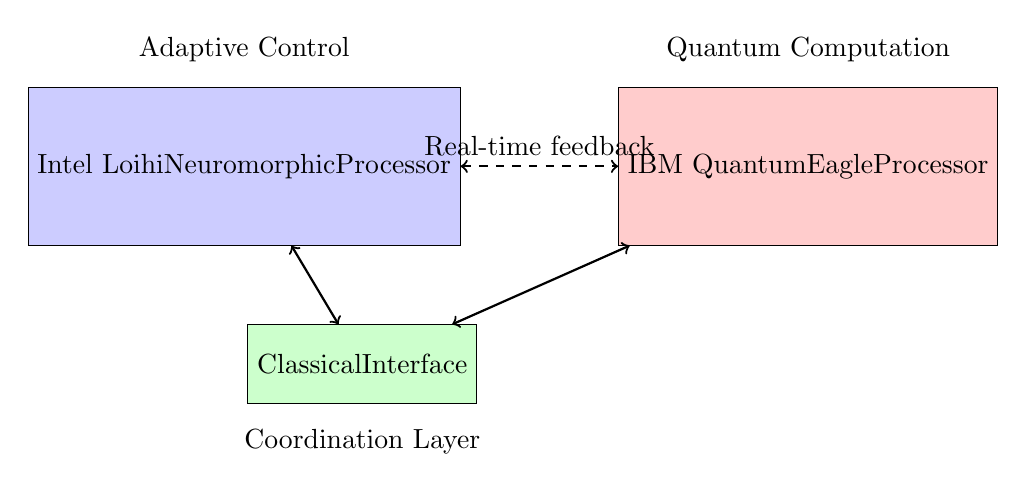
\begin{tikzpicture}[node distance=2cm]
% Neuromorphic processor
\node[draw, rectangle, minimum width=3cm, minimum height=2cm, fill=blue!20] (neuro) {Intel Loihi\\Neuromorphic\\Processor};

% Quantum processor  
\node[draw, rectangle, minimum width=3cm, minimum height=2cm, fill=red!20, right=of neuro] (quantum) {IBM Quantum\\Eagle\\Processor};

% Interface
\node[draw, rectangle, minimum width=2cm, minimum height=1cm, fill=green!20, below=1cm of neuro, xshift=1.5cm] (interface) {Classical\\Interface};

% Arrows
\draw[<->, thick] (neuro) -- (interface);
\draw[<->, thick] (quantum) -- (interface);
\draw[<->, thick, dashed] (neuro) -- (quantum) node[midway, above] {Real-time feedback};

% Labels
\node[above=0.2cm of neuro] {Adaptive Control};
\node[above=0.2cm of quantum] {Quantum Computation};
\node[below=0.2cm of interface] {Coordination Layer};
\end{tikzpicture}
\end{document}
